\begin{adjustwidth*}{}{-2.25in}
\textbf{{\large Exercises}}
\setlength{\columnsep}{25pt}
\begin{multicols*}{2}
%\noindent Terms and Concepts \small
%\begin{enumerate}[1)]
%\item blank
%\end{enumerate} 

\noindent {\normalsize Problems} \small

\begin{enumerate}[1)]
%Item 
\item Along the eastern shore of Lake Michigan from Lake Macatawa (near Holland) to Grand Haven, there is a bike path that runs almost directly north-south.  For the purposes of this problem, assume the road is completely straight, and that the function $s(t)$ tracks the position of the biker along this path in miles north of Pigeon Lake, which lies roughly halfway between the ends of the bike path.  
  
Suppose that the biker's velocity function is given by the graph below on the time interval $0 \le t \le 4$ (where $t$ is measured in hours), and that $s(0) = 1$.
\begin{center}
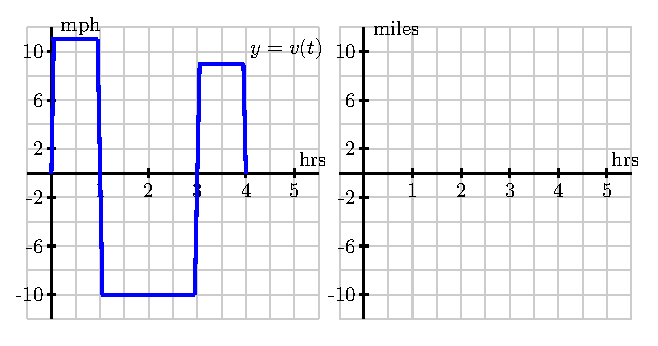
\includegraphics[scale=.6]{figures/4_1_Ez1.eps}
\end{center}
\ba
	\item Approximately how far north of Pigeon Lake was the cyclist when she was the greatest distance away from Pigeon Lake?  At what time did this occur?
	\item What is the cyclist's total change in position on the time interval $0 \le t \le 2$?  At $t = 2$, was she north or south of Pigeon Lake?
	\item What is the total distance the biker traveled on $0 \le t \le 4$?  At the end of the ride, how close was she to the point at which she started?
	\item Sketch an approximate graph of $y = s(t)$, the position function of the cyclist, on the interval $0 \le t \le 4$.  Label at least four important points on the graph of $s$.
\ea

%Item
\item A toy rocket is launched vertically from the ground on a day with no wind.  The rocket's vertical velocity at time $t$ (in seconds) is given by $v(t)= 500-32t$ feet/sec.
  \ba
  	\item At what time after the rocket is launched does the rocket's velocity equal zero?  Call this time value $a$.  What happens to the rocket at $t = a$?
	\item Find the value of the total area enclosed by $y = v(t)$ and the $t$-axis on the interval $0 \le t \le a$.  What does this area represent in terms of the physical setting of the problem?
	\item Find a function $s$ such that $s'(t) = v(t)$, or an antiderivative of $v(t)$.
	\item Compute the value of $s(a) - s(0)$.  What does this number represent in terms of the physical setting of the problem?
	\item Compute $s(5) - s(1)$.  What does this number tell you about the rocket's flight?
  \ea
  
%Item
  \item An object moving along a horizontal axis has its instantaneous velocity at time $t$ in seconds given by the function $v$ pictured below, where $v$ is measured in feet/sec.
\begin{center}
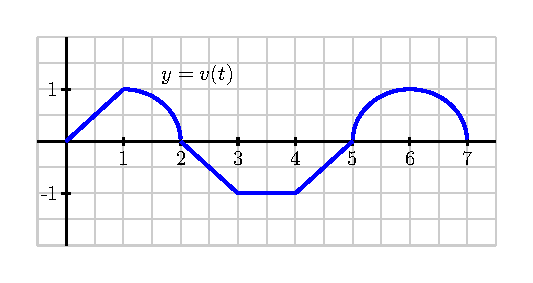
\includegraphics[scale=.75]{figures/4_1_Ez3.eps}
\end{center}
Assume that the curves that make up the parts of the graph of $y=v(t)$ are either portions of straight lines or portions of circles.
 \ba
 	\item Determine the exact total distance the object traveled on $0 \le t \le 2$.
	\item What is the value and meaning of $s(5) - s(2)$, where $y = s(t)$ is the position function of the moving object?
	\item On which time interval did the object travel the greatest distance: $[0,2]$, $[2,4]$, or $[5,7]$?
	\item On which time interval(s) is the position function $s$ increasing?  At which point(s) does $s$ achieve a relative maximum?
 \ea
 
%Item
  \item Filters at a water treatment plant become dirtier over time and thus become less effective; they are replaced every $30$ days.  During one $30$-day period, the rate, $p(t)$, at which pollution passes through the filters into a nearby lake (in units of particulate matter per day) is measured every $6$ days and is given in the following table.  The time $t$  is measured in days since the filters were replaced.
\begin{center}
\begin{tabular}{|l|c|c|c|c|c|c|}
\hline
Day, $t$ & $0$ & $6$ & $12$ &	$18$ & $24$ & $30$ \\
\hline
$p(t)$ & $7$ & $8$ & $10$ &	$13$ & $18$ & $35$ \\
\hline
\end{tabular}
\end{center}
\ba
	\item Plot the given data on a set of axes with time on the horizontal axis and the rate of pollution on the vertical axis.
	\item Explain why the amount of pollution that entered the lake during this $30$-day period would be given exactly by the area bounded by $y = p(t)$ and the $t$-axis on the time interval $[0,30]$.
	\item Estimate the total amount of pollution entering the lake during this $30$-day period.  Carefully explain how you determined your estimate.
\ea
\end{enumerate}

%------------------------------------------
% END OF EXERCISES ON FIRST PAGE
%------------------------------------------
\end{multicols*}
\end{adjustwidth*}

\clearpage

\begin{adjustwidth*}{}{-2.25in}
\setlength{\columnsep}{25pt}
\begin{multicols*}{2}\small

\noindent{\bf In Exercises 5--6, a graph of the velocity function of an object moving in a straight line is given.  Answer the questions based on the graph.}

\begin{enumerate}[1),start=5]
%ITEM
\item \begin{minipage}{\linewidth}
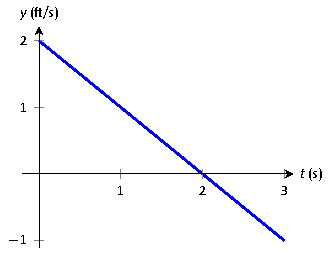
\includegraphics[scale=.8]{figures/fig05_02_ex_14}
\end{minipage}
\begin{enumerate}
\item		What is the object's maximum velocity?
\item		What is the object's maximum displacement?
\item		What is the object's total displacement on $[0,3]$?
\end{enumerate}

%ITEM
\item \begin{minipage}{\linewidth}
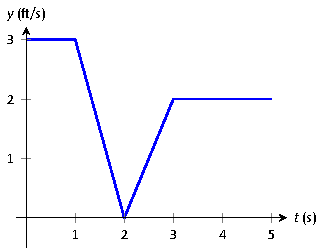
\includegraphics[scale=.8]{figures/fig05_02_ex_15}
\end{minipage}
\begin{enumerate}
\item		What is the object's maximum velocity?
\item		What is the object's maximum displacement?
\item		What is the object's total displacement on $[0,5]$?
\end{enumerate}

%ITEM 
\item An object is thrown straight up with a velocity, in ft/s, given by $v(t) = -32t+64$, where $t$ is in seconds, from a height of $48$ feet.
\begin{enumerate}
\item		What is the object's maximum velocity?
\item		What is the object's maximum displacement?
\item		When does the maximum displacement occur?
\item		When will the object reach a height of 0? (Hint: find when the displacement is $-48$ft.)
\end{enumerate}

%ITEM
\item An object is thrown straight up with a velocity, in ft/s, given by $v(t) = -32t+96$, where $t$ is in seconds, from a height of $64$ feet.
\begin{enumerate}
\item		What is the object's initial velocity?
\item		When is the object's displacement $0$?
\item		How long does it take for the object to return to its initial height?
\item		When will the object reach a height of $210$ feet?
\end{enumerate}
\end{enumerate}

%---------------------------------------------
% END OF EXERCISES ON SECOND PAGE
%---------------------------------------------
\end{multicols*}
\end{adjustwidth*}

\afterexercises